\section{Unifying Compostional Verification and Certified Compilation}
\label{sec:compcerto}

In this section we describe the core semantic framework
we propose to use for our approach to compositional verification.
%
Our framework consists of four kinds of objects,
each subject to some or all of four
different composition principles
(layered $\odot$,
 vertical $\fatsemi$,
 flat $\oplus$,
 spatial $\mathbin@$).
We start with a brief overview of how these constructions fit together,
then examine each one in more detail.

\subsection{Overview} %{{{

%{{{

Our model starts with a simple form of game semantics
built around the notion of \emph{effect signature} ($E, F\ldots$).
We use these signatures to describe the
interfaces between the components of a software system.
Effect signatures serve
as horizontal endpoints for \emph{strategies}
and vertical endpoints for \emph{refinement conventions}.
Strategies
($L : E \twoheadrightarrow F$)
describe the behaviors of program components.
Refinement conventions
($\mathbf{R} : E_1 \leftrightarrow E_2$)
model relationships between
views of the system at different levels of abstraction.
Finally,
\emph{refinement proofs}
($\phi : L_1 \le_{\mathbf{R} \rightarrow \mathbf{S}} L_2$)
connect the three kinds of objects above
in the shape of a square (Fig.~\ref{fig:hvcomp}).

%}}}

\vspace*{-2ex}
\paragraph{Composition principles} %{{{

Our framework uses
refinement squares as the building blocks of compositional proofs.
They are assembled in the manner of puzzle pieces
alongside matching edges:
\begin{itemize}
\item Layered composition ($\odot$) acts horizontally.
  It connects strategies at a common endpoint (\emph{ie.}~effect signature)
  over which they are made to interact,
  and connects refinement squares alongside a common
  vertical edge (\emph{ie.}~refinement convention),
  ensuring compatible abstractions and constraints.
  %assumptions of one refinement proof
  %are established as guarantees by the other.
\item Vertical composition ($\fatsemi$)
  combines successive refinement steps,
  connecting refinement conventions alongside an intermediate signature,
  and refinement squares along a common strategy,
  which serves as an intermediate specification.
\item Flat composition ($\oplus$)
  serves as an alternative form of horizontal composition
  where components are laid out side by side
  instead of being made to interact.
  We will not discuss it extensively.
\item Spatial composition ($\mathbin@$)
  equips our framework with infrastructure
  for compositional state.
\end{itemize}
We will examine each of these constructions in the remainder of this section.

%}}}

%}}}

\begin{figure} % fig:hvcomp {{{
  \[
  \begin{array}{c}
    \begin{tikzcd}[sep=0.5ex]
      E_1 \ar[dd, leftrightarrow, "\mathbf{R}"']
	  \ar[rr, "L_1"] &&
      F_1 \ar[dd, leftrightarrow, "\mathbf{S}"] \\
      & \phi & \\
      E_2 \ar[rr, "L_2"'] &&
      F_2
    \end{tikzcd}
  \end{array}
  \quad
  \begin{array}{c}
    \begin{prooftree}
      \hypo{L_1 : F \twoheadrightarrow G}
      \hypo{L_2 : E \twoheadrightarrow F}
      \infer2[\kw{ts}-$\odot$]{L_1 \odot L_2 : E \twoheadrightarrow G}
    \end{prooftree}
    \qquad
    \begin{prooftree}
      \hypo{\phi: L_1 \le_{\mathbf{S} \twoheadrightarrow \mathbf{T}} L_1'}
      \hypo{\psi: L_2 \le_{\mathbf{R} \twoheadrightarrow \mathbf{S}} L_2'}
      \infer2[\kw{sim}-$\odot$]{\phi \odot \psi :
	L_1 \odot L_2 \le_{\mathbf{R} \twoheadrightarrow \mathbf{T}} L_1' \odot L_2'}
    \end{prooftree}
    \\[1.5em]
    \begin{prooftree}
      \hypo{\mathbf{R} : E_1 \leftrightarrow E_2}
      \hypo{\mathbf{R}' : E_2 \leftrightarrow E_3}
      \infer2[\kw{sc}-$\vcomp$]{\mathbf{R} \vcomp \mathbf{R}' : E_1 \leftrightarrow E_3}
    \end{prooftree}
    \qquad
    \begin{prooftree}
      \hypo{\phi : L_1 \le_{\mathbf{R} \twoheadrightarrow \mathbf{S}} L_2}
      \hypo{\psi : L_2 \le_{\mathbf{R'} \twoheadrightarrow \mathbf{S'}} L_3}
      \infer2[\kw{sim}-$\vcomp$]{\phi \vcomp \psi : L_1 \le_{\mathbf{R} \vcomp \mathbf{R'} \twoheadrightarrow
	\mathbf{S} \vcomp \mathbf{S'}} L_3}
    \end{prooftree}
  \end{array}
\]
  \caption{Horizontal ($\odot$) and vertical ($\vcomp$)
    composition principles in our model.}
  \label{fig:hvcomp}
\end{figure}
%}}}

%\subsection{Game Semantics} \label{sec:gamesem} %{{{
%
%% preamble {{{
%
%Game semantics is a form of denotational semantics which
%incorporates some operational aspects,
%and which heavily informs the design of CompCertO.
%We start with an exposition of its basic tenets,
%and how we deploy them to prove the compositional correctness of CompCert.
%
%%An early success of this approach was
%%the formulation of the first fully abstract models
%%of the programming language PCF \cite{pcfajm,pcfho}.
%%In this section,
%%we give an overview of this line of research
%%and how it can be applied in the context of CompCert.
%Typically,
%game semantics interpret
%\emph{types} as two-player games
%and \emph{terms} as strategies for these games.
%The games describe the form of the interaction
%between a program component %of the corresponding type
%(the \emph{system})
%and its execution context
%(the \emph{environment}).
%Strategies
%specify which move the system plays
%for each possible configuration of the game.
%Configurations are usually identified with sequences of moves
%(\emph{plays}),
%and strategies with the set of configurations
%a component can reach.
%
%%This representation makes
%%game semantics similar to
%%the trace semantics of process algebras,
%%but game semantics is distinguished
%%by a strong polarization between
%%the actions of the system and those of the environment.
%%%and between outputs and inputs.
%%This confers an inherent ``rely-guarantee'' flavor
%%to games which facilitates compositional reasoning
%%\cite{cspgs}.
%
%%}}}
%
%\vspace*{-2ex}
%\paragraph{Games} \label{sec:mainideas:gs:games} %{{{
%A game is defined by a set of moves
%players will choose from,
%as well as a stipulation of which
%sequences of moves are valid.
%We focus on two-player, alternating games
%where the environment plays first and
%where the players
%each contribute every other move.
%When typesetting examples,
%we underline the moves of the system.
%For example, a valid play for Black in the game of chess may look like:
%%For chess,
%%moves are taken in the set $\{a1 \ldots h8\} \times \{a1 \ldots h8\}$,
%%and a valid sequence of moves may look like:
%\[ e2e4 \cdot \underline{c7c5} \cdot c2c3 \cdot \underline{d7d5} \cdots \]
%Game semantics allows
%simple games to be combined into more sophisticated ones,
%which can then be used
%to interpret compound types.
%For example,
%in the game $A \times B$
%the environment initially chooses whether to play
%an instance of $A$ or an instance of $B$.
%The game $A \rightarrow B$ usually consists of
%an instance of $B$ played
%together with instances of $A$
%started at the discretion of the system,
%where the roles of the players are reversed.
%%and which correspond to
%%the multiple accesses to the argument values
%%allowed by most $\lambda$-calculi.
%%}}}
%
%%}}}

\subsection{Effect Signatures} \label{sec:esig} %{{{

%The games we use are particularly simple.
Like interaction trees \cite{itrees},
our model uses \emph{effect signatures}
%\citep{some-algebraic-effects-ref}
to describe interfaces between system components.
An effect signature enumerates
the external operations which
a component can invoke or implement,
and describes for each one
the set of possible outcomes.

\begin{definition} \label{def:esig}
An \emph{effect signature} is a set $E$ of \emph{questions}
together with an assignment $\kw{ar} : E \rightarrow \mathbf{Set}$
associating to each question $m \in E$
a set of \emph{answers} $n \in \kw{ar}(m)$.
We will often present them together as the set of bindings
$\{ (m \mathbin: N) \mid m \in E \wedge N = \kw{ar}(m) \}$.
%$\{ m \mathbin: \kw{ar}(m) \}_{m \in E}$.
\end{definition}

%In the algebraic effects literature,
%a question $m \mathbin: N$ in a signature $E$ is interpreted as
%an algebraic operation of arity $N$, representing a possible effect.
%The term $m(k_i)_{i \in N}$ is then a computation
%which triggers the effect $m$ with possible continuations $k_i$.
%In our case,
%%We revisit this algebraic interpretation in~\S\ref{sec:model},
%%but for now
%we will focus on effect signatures as elementary games.

\begin{example}[CompCertO language interfaces] \label{ex:compcertosig} %{{{

The CompCertO semantics for the C language
rely on an effect signature $\mathcal{C} \mathbin@ \kw{mem}$.
Questions are function calls;
they take the form of a (stylized) tuple $f(\vec{v})@m$, where
$f$ identifies the function to be called,
$\vec{v} \in \kw{val}^*$ are the actual parameters, and
$m \in \kw{mem}$ is the memory state at the time of invocation;
answers take the form $v'@m'$ where
$v' \in \kw{val}$ is value returned by the function~$f$ and
$m' \in \kw{mem}$ is the new state of the memory.
This is captured by the effect signature
\[
  \mathcal{C} \mathbin@ \kw{mem} \:=\:
  \{ f(\vec{v})@m \mathbin: \kw{val} \times \kw{mem} \mid
     f \in \kw{val}, \:
     \vec{v} \in \kw{val}^*, \:
     m \in \kw{mem} \}
  \,.
\]
We will elucidate the structure of
the spatial decomposition $\mathcal{C} \mathbin@ \kw{mem}$ below.
\end{example}
%}}}

%}}}

\begin{figure} % fig:overview:ts {{{
  \begin{subfigure}{0.35\textwidth}
    \centering
    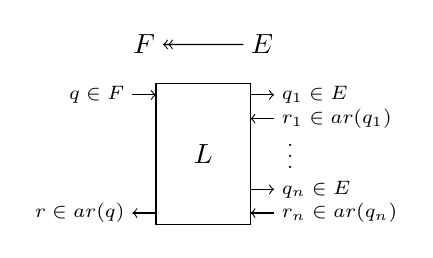
\begin{tikzpicture}[yscale=0.15,xscale=0.30]
      \draw (1,-1) rectangle (5,11) node[midway] {$L$};
      \scriptsize
      \draw[->] (0,10) node[left] {$q \in F$} -- (1,10)
          node[above=1.5em,midway] (B) {\normalsize $F$};
        \draw[->] (5,10) -- (6,10) node[right] {$q_1 \in E$}
          node[above=1.5em,midway] (A) {\normalsize $E$};
        \draw[->] (6,8) node[right] {$r_1 \in \kw{ar}(q_1)$} -- (5,8) ;
        \node[right] at (6,5.5) {$\:\vdots$};
        \draw[->] (5,2) -- (6,2) node[right] {$q_n \in E$};
        \draw[->] (6,0) node[right] {$r_n \in \kw{ar}(q_n)$} -- (5,0);
      \draw[->] (1,0) -- (0,0) node[left] {$r \in \kw{ar}(q)$};
      \draw[->>] (A) -- (B);
    \end{tikzpicture}
    \subcaption{General shape}
    \label{fig:overview:ts:shape}
  \end{subfigure}
  \begin{subfigure}{0.30\textwidth}
    \centering
    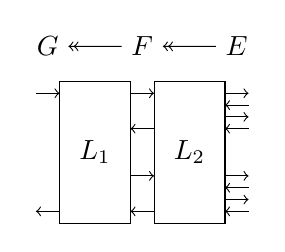
\begin{tikzpicture}[yscale=0.15,xscale=0.30]
      \draw (1,-1) rectangle (4,11) node[midway] {$L_1$};
      \draw (5,-1) rectangle (8,11) node[midway] {$L_2$};
      %\draw (5,-1) rectangle (8,4) node[midway] {$L_2$};
      \draw[->] (0,10) -- (1,10) node[above=1em,midway] (C) {$G$};
        \draw[->] (4,10) -- (5,10) node[above=1em,midway] (B) {$F$};
          \draw[->] (8,10) -- (9,10) node[above=1em,midway] (A) {$E$};
          \draw[->] (9,9) -- (8,9);
          \draw[->] (8,8) -- (9,8);
          \draw[->] (9,7) -- (8,7);
        \draw[->] (5,7) -- (4,7);
        \draw[->] (4,3) -- (5,3);
          \draw[->] (8,3) -- (9,3);
          \draw[->] (9,2) -- (8,2);
          \draw[->] (8,1) -- (9,1);
          \draw[->] (9,0) -- (8,0);
        \draw[->] (5,0) -- (4,0);
      \draw[->] (1,0) -- (0,0);
      \draw[->>] (A) -- (B);
      \draw[->>] (B) -- (C);
    \end{tikzpicture}
    \subcaption{Composition}
    \label{fig:overview:ts:comp}
  \end{subfigure}
  \begin{subfigure}{0.25\textwidth}
    \centering
    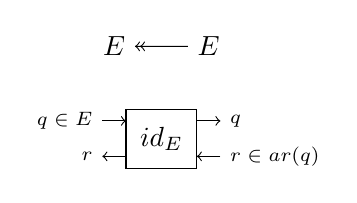
\begin{tikzpicture}[yscale=0.15,xscale=0.30]
      \draw (5,-1) rectangle (8,4) node[midway] {$\kw{id}_E$};
      \draw[->] (4,3) node[left] {\scriptsize $q \in E$}
             -- (5,3) node[above=2em,midway] (A2) {$E$};
        \draw[->] (8,3) -- (9,3) node[above=2em,midway] (A1) {$E$}
                                 node[right] {\scriptsize $q$};
        \draw[->] (9,0) node[right] {\scriptsize $r \in \kw{ar}(q)$} -- (8,0);
      \draw[->] (5,0) -- (4,0) node[left] {\scriptsize $r$};
      \draw[->>] (A1) -- (A2);
    \end{tikzpicture}
    \vspace{1ex}
    \subcaption{Identity}
    \label{fig:overview:ts:id}
  \end{subfigure}
  \caption{Informal description of our strategy model
    under \emph{layered} composition}  
  \label{fig:overview:ts}
\end{figure}
%}}}

\subsection{Strategies} \label{sec:strat} %{{{

We use effect signatures to assign coarse types
to program components and to their behaviors.
Specifically,
a~\emph{strategy} $L : E \twoheadrightarrow F$
models the behavior of a component which
uses operations of the signature $E$ to
implement the operations enumerated in $F$.

As depicted in Fig.~\ref{fig:overview:ts}a,
the environment can activate $L$ by asking a question $q \in F$,
which the component $L$ is expected to eventually answer
with a reply $r \in \kw{ar}(q)$.
In the process,
$L$ can perform an arbitrary number of queries $q_i \in E$,
which the environment answers with a response $r_i \in \kw{ar}(q_i)$.
The process can then begin anew with a question $q' \in F$,
and so on indefinitely.
We will write
\[
  L \:\vDash\: \big(q
    \rightarrowtail (m_1 \leadsto n_1)
    \rightarrowtail (m_2 \leadsto n_2)
    \rightarrowtail \cdots
    \rightarrowtail (m_k \leadsto n_k)
    \rightarrowtail r \big)
  \leadsto \big(q'
    \rightarrowtail \cdots
    \rightarrowtail r' \big)
  \leadsto \cdots
\]
to mean that $L$ accepts an execution trace of this kind.
Note that $\rightarrowtail$ denotes a part of the execution
where $L$ is in control,
whereas $\leadsto$ denotes a part of the execution
controlled by the environment.

\begin{figure} % fig:abc {{{
  \figsize
  \centering
  \tt
  {\footnotesize
  \begin{tabular}{ll lr@{\ }l}
    \hline
    \underline{A.c} & int mult(n, p) \{ &
    \underline{A.s} & mult: & \%eax := \%ebx \\
                    & \quad return n * p; &
                    & & \%eax *= \%ecx \\
                    & \} &
                    & & ret \\
    \hline
    \underline{B.c} & int sqr(n) \{ &
    \underline{B.s} & sqr: & \%ecx := \%ebx \\
                    & \quad return mult(n, n); &
                    & & call mult \\
                    & \} &
                    & L: & ret \\
    \hline
  \end{tabular}
  }
  \caption{Two simple C compilation units and corresponding assembly code.
    For this example,
    the calling convention stores arguments in
    the registers
    \texttt{\%ebx} and \texttt{\%ecx}
    and return values in
    the register
    \texttt{\%eax}.}
  \label{fig:abc}
\end{figure}
%}}}

\begin{example}[CompCertO semantics] \label{ex:compcertosem} %{{{
We described in Example~\ref{ex:compcertosig}
the signature $\mathcal{C} \mathbin@ \kw{mem}$
used in CompCertO for C-level function calls and returns.
By the same token, CompCertO language semantics
can be described as strategies.
For example,
the source language used by CompCertO
is a simplified version of~C called Clight,
and its semantics for a program $M$ can be used to define:
$
  \kw{Clight}(M) : \mathcal{C} \mathbin@ \kw{mem}
    \twoheadrightarrow \mathcal{C} \mathbin@ \kw{mem}
$.
Referring to the code in Fig.~\ref{fig:abc},
the resulting strategies will exhibit traces such as:
\begin{align*}
  \kw{Clight}(\kw{A.c}) \:&\vDash\:
  \kw{sqr}(2)@m \rightarrowtail
  (\kw{mult}(2,2)@m \leadsto 4@m) \rightarrowtail
  4@m \,,
\\
  \kw{Clight}(\kw{B.c}) \:&\vDash\:
  \kw{mult}(2,2) \rightarrowtail 4
  \,.
\end{align*}
Note that the programs are simple enough that
their execution does not alter the memory state $m$.
\end{example}
%}}}

%}}}

\subsection{Layered Composition} %{{{

When a component $L_1 : F \twoheadrightarrow G$
uses an interface $F$ implemented by
another component $L_2 : E \twoheadrightarrow F$,
we can direct the questions asked by $L_1$ in $F$ to $L_2$
(Fig.~\ref{fig:overview:ts}b).
The result is the composite strategy
$L_1 \odot L_2 : E \twoheadrightarrow G$. %(Def.~X.Y).
This is the main form of horizontal composition which we will be using.

\begin{example}[Composing C programs] %{{{
Referring once again to Fig.~\ref{fig:abc},
the semantics of the two components can be composed
to yield traces such as:
\[
  \kw{Clight}(\kw{B.c}) \odot \kw{Clight}(\kw{A.c})
  \vDash
  \kw{sqr}(2)@m \rightarrowtail 4@m
  \,.
\]
\end{example}

\begin{example}[Layer Interfaces] \label{ex:calcomp} %{{{
The \emph{certified abstraction layers} (CAL) methodology used to verify
the CertiKOS operating system kernel \cite{dscal15}
involves a notion of \emph{underlay interface},
which provides specifications for the primitives which
code at a certain level of abstraction is able to rely on.

In our framework, a layer interface is a strategy of type:
$
  L : \emptysig \twoheadrightarrow \mathcal{C} \mathbin@ \kw{mem} \mathbin@ D
$,
where the signature $0$ is empty,
and $\mathcal{C} \mathbin@ \kw{mem} \mathbin@ D$
extends the CompCert memory model $\kw{mem}$
with an \emph{abstract state} component of type $D$.
The CompCertO semantics of a program component $M$ can be lifted to
$
  \kw{Clight}(M) \mathbin@ D \: : \:
    \mathcal{C} \mathbin@ \kw{mem} \mathbin@ D \: \twoheadrightarrow \:
    \mathcal{C} \mathbin@ \kw{mem} \mathbin@ D
$
to keep track of of this additional state component. 
We can then evaluate the effect of running $M$
on top of the underlay interface $L$ as the strategy:
\[
  (\kw{Clight}(M) \mathbin@ D) \odot L \: : \:
    \emptysig \: \twoheadrightarrow \:
    \mathcal{C} \mathbin@ \kw{mem} \mathbin@ D
    \,.
\]
\end{example}
%}}}

%}}}

\subsection{Refinement Conventions and Refinement Squares} \label{sec:sconv} %{{{

High-level specifications given in abstract terms
are often implemented in lower-level terms.
For example, the specification of a NAND logic gate
is usually given as a truth table,
but its realization as an integrated circuit
deals in voltages and currents.
This is possible because some kind of \emph{convention}
establishes the connection between
the high- and low-level views of a component---%
for example, a logic family like TTL or CMOS
will specify which voltage ranges correspond
to the logic levels 0 and 1.

In our setting, this idea is formalized
as the notion of \emph{refinement convention} between effect signatures.
Then a refinement property
$\phi : L_1 \le_{\mathbf{R} \rightarrow \mathbf{S}} L_2$,
which asserts that the high-level specification $L_1$
is realized by the low-level implementation $L_2 : E_2 \twoheadrightarrow F_2$,
is parameterized by two refinement conventions
$\mathbf{R} : E_1 \leftrightarrow E_2$ and
$\mathbf{S} : F_1 \leftrightarrow F_2$.
The corresponding refinement property assumes that incoming
source- and target-level questions in $F_1$ and $F_2$
will be related according to the convention $\mathbf{S}$,
and guarantees that outgoing questions in $E_1$ and $E_2$
will be related according to $\mathbf{R}$.
Conversely, it assumes that
the environment's answers in $E$
will be related according to $\mathbf{R}$
and guarantees that the components' answers in $F$
will be related according to $\mathbf{S}$.

\begin{example}[Semantics preservation of CompCert] %{{{
\label{ex:bq-proof}
Compilers operate in the context of a \emph{calling convention},
which specify how C-level calls are realized
in terms of low-level, architecture-specific assembly language constructs.
In CompCertO,
the compiler's correctness theorem involves
a convention
$\mathbb{C} : \mathcal{C} \leftrightarrow \mathcal{A}$,
which is used to express the way in which
C-level function calls ($\mathcal{C}$) are encoded
as assembly-level interactions ($\mathcal{A}$).
the correctness proof of CompCertO
can then be put in the form of a refinement square:
\[
  \kw{CompCert}(p) = p'
  \quad \Longrightarrow \quad
    \phi^\kw{cc}_p :
      \kw{Clight}(p) \le_{\mathbb{C} \twoheadrightarrow \mathbb{C}} \kw{Asm}(p')
\]
where %the refinement convention
$\mathbb{C} : \mathcal{C} \leftrightarrow \mathcal{A}$
models the calling convention used by CompCert.
Assuming the code in Fig.~\ref{fig:abc} uses a compatible calling convention,
we would be able to prove as well:
\[
  \kw{Clight}(\kw{A.c}) \le_{\mathbb{C} \twoheadrightarrow \mathbb{C}} \kw{Asm}(\kw{A.s})
  \quad \text{and} \quad
  \kw{Clight}(\kw{B.c}) \le_{\mathbb{C} \twoheadrightarrow \mathbb{C}} \kw{Asm}(\kw{B.s})
  \,,
\]
establishing these refinements as compatible.
In other words,
because they use the same conventions,
these refinement squares can all be combined,
and as a result we can prove that
linking C source code with $\kw{A.c}$
would have a similar effect as linking the corresponding CompCert-compiled code with $\kw{A.s}$.
\end{example}
%}}}

\begin{example}[Layer Implementations] %{{{
In the context of CAL (Example~\ref{ex:calcomp}),
code running on an \emph{underlay} interface
$L : \emptysig \twoheadrightarrow \mathcal{C} \mathbin@ \kw{mem} \mathbin@ D$
is ultimately shown to implement an \emph{overlay} interface
$L' : \emptysig \twoheadrightarrow \mathcal{C} \mathbin@ \kw{mem} \mathbin@ D'$.
To this end, we must first provide a relation
$R \subseteq (\kw{mem} \times D) \times (\kw{mem} \times D')$
which establishes a correspondence between
the more abstract overlay states and more concrete underlay states.
This relation can be used to define a refinement convention
$\mathcal{C} \mathbin@ R : \mathcal{C} \mathbin@ \kw{mem} \mathbin@ D
 \leftrightarrow \mathcal{C} \mathbin@ \kw{mem} \mathbin@ D'$
and express the layer correctness property as a refinement square
\[
  L \vdash_R M : L' \quad :\Longleftrightarrow \quad
  L' \, \le_{\emptysig \twoheadrightarrow \mathcal{C} \mathbin@ R} \,
    (\kw{Clight}(M) \mathbin@ D) \odot L
  \,.
\]
The composition properties of our framework can then be used to establish that
two successive layer implementations
$L \vdash_R M : L' \vdash_S N : L''$ can be combined into a single layer
$L \vdash_{R \mathbin; S} M N : L''$.
Note that we have used $\emptysig$ to denote the identity refinement convention
for the effect signature of the same name. 
\end{example}
%}}}

%}}}

\subsection{Spatial Composition} \label{sec:scomp} %{{{

The notation $X \mathbin@ Y$ which we have used informally
denotes \emph{spatial composition}.
For an effect signature $E$ and a set $U$
we can define the composite effect signature:
\[
  E \mathbin@ U \: := \:
    \{ m @ u : N \times U \mid (m : N) \in E \}
  \,,
\]
which annotates every question and every answer of $E$
with an additional component of type $U$.
Spatial composition extends to strategies,
refinement conventions and refinement squares
as depicted in Fig.~\ref{fig:xcomp}.

\begin{figure} % fig:xcomp {{{
  \begin{gather*}
    \begin{prooftree}
      \hypo{L : A \twoheadrightarrow B}
      \hypo{f : U \lensarrow V}
      \infer2[\kw{ts}-$\mathbin@$]{
        L \mathbin@ f : A \mathbin@ U \twoheadrightarrow B \mathbin@ V
      }
    \end{prooftree}
    \hspace{8em}
    \begin{prooftree}
      \hypo{\mathbf{R} : A \leftrightarrow B}
      \hypo{\mathbf{S} : U \leftrightarrow V}
      \infer2[\kw{sc}-$\mathbin@$]{
        \mathbf{R} \mathbin@ \mathbf{S} : A \mathbin@ U \leftrightarrow B \mathbin@ V
      }
    \end{prooftree}
%    \\[1em]
%    \begin{array}{r@{}l}
%      (L_1 \odot L_2) \mathbin@ (f \circ g) & {} \equiv
%      (L_1 \mathbin@ f) \odot (L_2 \mathbin@ g) \\
%      \kw{id}_A \mathbin@ \kw{id}_U & {} \equiv \kw{id}_{A \mathbin@ U}
%    \end{array}
%    \quad
%    \begin{array}{r@{}l}
%      (\mathbf{R}_1 \vcomp \mathbf{R}_2) \mathbin@ (\mathbf{S}_1 \vcomp \mathbf{S}_2)
%      & {} \equiv
%      (\mathbf{R}_1 \mathbin@ \mathbf{S}_1) \vcomp (\mathbf{R}_2 \mathbin@ \mathbf{S}_2)
%      \\
%      \idsc_A \mathbin@ \idsc_U & {} \equiv \idsc_{A \mathbin@ U}
%    \end{array}
    \\[1em]
    \begin{prooftree}
      \hypo{\phi: L \le_{\mathbf{R}_1 \twoheadrightarrow \mathbf{S}_1} L'}
      \hypo{\psi: f \le_{\mathbf{R}_2 \twoheadrightarrow \mathbf{S}_2} f'}
      \infer2[\kw{sim}-$\mathbin@$]{\phi \mathbin@ \psi :
	L \mathbin@ f
        \le_{\mathbf{R}_1 \mathbin@ \mathbf{R}_2 \twoheadrightarrow
             \mathbf{S}_1 \mathbin@ \mathbf{S}_2}
	L' \mathbin@ f'}
    \end{prooftree}
  \end{gather*}
  \caption{Spatial composition ($\mathbin@$) for strategies,
    simulation conventions and simulation proofs.}
  \label{fig:xcomp}
\end{figure}
%}}}

\vspace*{-2ex}
\paragraph{Strategies}

A strategy of type $\sigma : E \twoheadrightarrow F$
can be extended to act on an additional state component
by specifying a transformation $f : U \lensarrow V$
between two sets $U$ and $V$
(transformations are specified using a form of stateful \emph{lenses}).
The result is a strategy
$\sigma \mathbin@ f : E \mathbin@ U \twoheadrightarrow F \mathbin@ V$.
The special case
$\sigma \mathbin@ U : E \mathbin@ U \twoheadrightarrow F \mathbin@ U$
used in Example~\ref{ex:calcomp}
relies on the identity transformation for the set $U$.
It simply passes along a state component of type $U$
in the questions and answers handled by $\sigma$
without modifying it directly.

\vspace*{-2ex}
\paragraph{Refinement Conventions and Refinement Squares}

The refinement convention
$\mathbf{R} \mathbin@ S : E \mathbin@ U \leftrightarrow F \mathbin@ V$
extends the convention $\mathbf{R} : E \leftrightarrow F$
with a plain relation $S \subseteq U \times V$
(more sophisticated forms of history-dependent relations can be used as well).
It expects the original part of questions and answers
to be related according to $\mathbf{R}$,
while the additional state components are related according to $S$.
A strategy and an associated state transformation 
can be refined independently
using two different refinement squares,
which can then be combined using the rule $\kw{sim}$-$@$
shown in Fig.~\ref{fig:xcomp}.

\vspace*{-2ex}
\paragraph{State Encapsulation}

One particularly interesting form of state transformation
is the \emph{encapsulation primitive}
$[u\rangle : U \lensarrow \mathbbm1$,
which hides a state component of type $U$.
On its first activation with a question component ${*} \in \mathbbm{1}$,
the encapsulation primitive reveals the initial state $u \in U$.
When an updated state $u' \in U$ is received,
the primitive stores the updated state for the next activation
and hides it again behind the trivial value ${*} \in \mathbbm{1}$.

\begin{example}[Hiding abstract state]
This allows us to hide the abstract state $D$
used by a layer interface $L$ by providing and initial value $d_0$
in the composite
$
  (\mathcal{C} \mathbin@ \kw{mem} \mathbin@ [d_0\rangle) \odot L :
  \emptysig \twoheadrightarrow \mathcal{C} \mathbin@ \kw{mem}
$.
The properties of our framework allow us to show that
hiding the abstract data first, then composing with $\kw{Clight}(M)$,
or composing first with $\kw{Clight}(M)\mathbin@ D$ then hiding the data,
yield equivalent results.
\end{example}

Moreover, a form of \emph{representation independence}
can be expressed in the form of a refinement square.
Specifically,
when then initial states $d_0 \mathrel{R} d_0'$
are related by $R \subseteq D \times D'$,
we can derive the property
$
  [d_0 \rangle \le_{R \twoheadrightarrow \mathbbm1} [d_0'\rangle
$,
which allows a refinement to take place between components
using different kinds of internal, hidden states
as long as a simulation relation can be established between them.

\vspace*{-2ex}
\paragraph{Memory Separation}

Spatial composition can also be used to formalize
certain \emph{memory separation} properties found in separation logic.
Specifically,
we were able to define a separation algebra for the CompCert memory model $\kw{mem}$,
and derive from it a refinement convention
$\mathbf{Y} : \kw{mem} \times \kw{mem} \leftrightarrow \kw{mem}$.
This convention can in turn be use to express the frame rule
for CompCert languages using refinement squares such as:
\[
  \kw{Clight}(M) \mathbin@ \kw{mem} \le_{\mathcal{C} \mathbin@ \mathbf{Y} \twoheadrightarrow
  \mathcal{C} \mathbin@ \mathbf{Y}} \kw{Clight}(M)
\]
Here, a view of the system where an additional memory share
is transparently passed alongside the execution of $M$ (but does not interact with it)
is refined by a lower-level view where this share
has been merged into the global memory state used by $\kw{Clight}$. 
The refinement shows that incorporating this additional memory share
does not alter any executions which were already possible without it,
in which case the additional share will moreover be left unchanged by $M$.
In the context of CAL,
this allows components of the abstract state
to be progressively refined into additional memory shares
to be incorporated into the global concrete memory state.

%}}}

\subsection{Proposed Work}

We have outlined the main features of a compositional framework
capable of capturing under a uniform notion of refinement square
a wide variety of properties:
\begin{itemize}
  \item code verification properties used to construct certified abstraction layers;
  \item the correctness property of the certified compiler CompCertO;
  \item representation independence properties associated with state encapsulation;
  \item the frame rule of separation logic.
\end{itemize}
In preliminary work,
we have shown that these different properties
can be fruitfully interfaced and assembled in the manner of puzzle pieces
to construct sophisticated refinement proofs.
%For example,
%a specification's encapsulated state
%can be made visible and refined into a concrete memory share,
%in order to prove a C program correct in the context of a particular data representation.
%The CompCertO correctness theorem can then be incorporated
%in order to transfer this property to the level of assembly code.
%
We seek to use this approach
to bridge the broader gap between
compositional \emph{certified compilation} on one hand, and
compositional \emph{verification} on the other hand.
When all is said and done,
our work will provide a three-dimensional algebra of refinement,
where correctness properties and high-level reasoning principles
can be expressed as simulation ``cubes''
which can be composed horizontally, vertically and spatially.
%Below we outline the work required to establish this foundation.

\vspace*{-2ex}
\paragraph*{Task 1a: Formalizing Categorical Structures}

Under $\odot$ and $\vcomp$,
strategies, simulation conventions and simulation proofs
constitute a \emph{double category},
a well-known structure equipped with a formal string diagram algebra
\cite{dcsd}.
By making explicit the underlying categorical structures
of our model,
we hope to facilitate connections with more theoretical work,
gain reasoning tools such as string diagrams,
and facilitate the modeling of heterogeneous systems
of the kind illustrated by Example~\ref{ex:nicdriver}.
A categorical characterization of our framework
would also provide a clean foundation for its mechanization
as a Coq library.

\vspace*{-2ex}
\paragraph*{Task 1b: Mechanizing our Compositional Semantics Framework}

We were able in preliminary work to mechanize the material presented here
into the Coq proof assistant.
However,
work remains to be done to obtain a production-quality Coq library
and provide a solid foundation for the extensions and applications
we intend to build on top of it,
as described in the remainder of this document.
We intend to release this library as open source code,
allowing other researchers to reuse and build on our work.

\vspace*{-2ex}
\paragraph*{Task 1c: Integrate CompCertO into the framework}

We have verified that the open transition system model used in CompCertO,
and the associated correctness proof,
can be embedded into the framework outlined in this section.
Once Task 1b is complete,
we will need to to ensure that CompCertO is integrated into our library
such that its language semantics and correctness theorem can be used
as easily as possible.
As part of this task,
we will seek to provide facilities
to help users connect high-level, abstract signatures and specifications
to lower-level C calls and their corresponding implementations.

